\documentclass[a4paper, 10pt]{article}
\usepackage[utf8]{inputenc} % Change according your file encoding
\usepackage{graphicx}
\usepackage{url}
\usepackage{amsmath}
\usepackage{amsthm}
\usepackage{algorithm}
\usepackage{multicol}
\usepackage[noend]{algpseudocode}
\usepackage{tikz}
\usetikzlibrary{shapes.geometric,positioning}
\usepackage[a4paper, left=2cm, right=2cm, top=2cm, bottom=2cm]{geometry}

\newtheorem{obs}{Observation}

%opening
\title{Seminar Report: [seminar ID] (e.g. Paxy)}
\author{\textbf{Name of team members}}
\date{\normalsize\today{}}

\begin{document}

% New definitions
\algnewcommand\algorithmicswitch{\textbf{switch}}
\algnewcommand\algorithmiccase{\textbf{case}}
\algnewcommand\algorithmicassert{\texttt{assert}}
\algnewcommand\Assert[1]{\State \algorithmicassert(#1)}%
% New "environments"
\algdef{SE}[SWITCH]{Switch}{EndSwitch}[1]{\algorithmicswitch\ #1\ \algorithmicdo}{\algorithmicend\ \algorithmicswitch}%
\algdef{SE}[CASE]{Case}{EndCase}[1]{\algorithmiccase\ #1}{\algorithmicend\ \algorithmiccase}%
\algtext*{EndSwitch}%
\algtext*{EndCase}%

%\maketitle
Carlos Segarra \hfill Thursday, September 26th

\vspace{15pt}

\textbf{\Large Discrete and Algorithmic Geometry: Problems 4 and 5}

\vspace{20pt}

\textbf{\textit{4. Propose an algorithm that, given a point $p$ external to a convex polygon $\mathcal{P}$, finds the point of $\mathcal{P}$ closest to $p$. What happens if instead of finding the closest point we look for the farthest? What if we restrict the search to the vertices of $\mathcal{P}$?}}

\vspace{3pt}

Let $\lbrace q_1, \dots, q_n\rbrace$ be the set of vertices of $\mathcal{P}$ in clock-wise order. And let $d_p$ be the function s.t. for all $q \in \mathcal{P}$, sends $p$ to $d(q, p)$. Before starting with the proof, let us make two observations:
\begin{obs}
    $d_p$ is an uni-modal application. Alternatively, its derivative is a linear funcion that has only one zero.
\end{obs}
\begin{obs} \label{obs-2}
    Let $q_{min}$ and $q_{min+1}$ be the closest and second to closest vertices from $\mathcal{P}$ to $p$. Then, the closest point in $\mathcal{P}$ to $p$ is either (i) $q_{min}$ or (ii) contained in the $q_{min}q_{min+1}$ segment.
\end{obs}

Note that the second observation applies symetrically to the farthest point in $\mathcal{P}$. 
Further, once we find the two closest points, checking wether we are in case (i) or case (ii) from Obs~\ref{obs-2} can be done in constant time testing if $p$ belongs to the triangle drawn by the line throguh $p$ parallel to $q_{min}q_{min+1}$ and the two lines through $p_{min}$ orthogonal to the segments incident to $p_{min}$.

To solve the problem we measure the increase in distance between the two starting points and the two in the middle, and apply binary search from there. The different cases, together with the decision of the final point are depicted in the figure below.

\tikzset{
  my poly/.style={regular polygon, regular polygon sides=6,fill=gray!#1,minimum size=2cm, draw},
}

\begin{figure}[h!]
    \resizebox{\linewidth}{!}{
    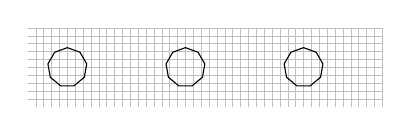
\begin{tikzpicture}[node distance=0pt, every node/.style={outer sep=0pt}]
        \draw [help lines,gray!50,step =0.1] (-0.5,-0.5) grid (4,0.5);
      %\node (1-C1) [my poly=10] {C1};
        \node (poly) [regular polygon, regular polygon sides=9, draw, minimum size = 0.5cm] at (0,0) {};
        \node (poly) [regular polygon, regular polygon sides=9, draw, minimum size = 0.5cm] at (1.5,0) {};
        \node (poly) [regular polygon, regular polygon sides=9, draw, minimum size = 0.5cm] at (3,0) {};
        %\fill[red] at (0.7, 0.2) circle (1pt);
        %\node[fill=red, minimum size = 0.01cm] at (0.7, -0.2) {};
      %\foreach \i/\j/\k/\m in {4/2/2/30,3/1/3/10,2/6/4/10,1/5/5/10,6/4/6/10,5/3/7/10}
      %\node (1-C\k) [my poly=\m, anchor=corner \i] at (1-C1.corner \j) {C\k};
    \end{tikzpicture}}
\end{figure}

Below, we include the Algorithm for computing the closest point to a polygon, note that, in order to find the farthest we could use the same exact algorithm
\begin{algorithm}
    \caption{Given a polygon $\mathcal{P}$ given by its vertices $\lbrace q_1, \dots, q_n\rbrace$ and a point $p$, find the closest point in $\mathcal{P}$ to $p$. \label{alg:closest}}
  \begin{multicols}{2}
  \begin{algorithmic}[1]
    %\Procedure{T-DAG Generation}{$s$}
        \State $start \gets 1$
        \State $end \gets \frac{n}{2}$
        \While{$start \leq end$}
            \State $\Delta_A \gets d_p(q_{start + 1}) - d_p(q_{start})$
            \State $\Delta_B \gets d_p(q_{end + 1}) - d_p(q_{end})$
            \Switch{$\text{sign}(\Delta_A)\text{, sign}( \Delta_B)$}
                \Case{$+ +$}
                    \State $\text{swap}(start, end)$ 
                \EndCase
                \Case{$+ -$}
                    \State $start \gets end$ 
                    \State $end \gets end + \frac{end - start}{2}$
                \EndCase
                \Case{$- +$}
                    \State $end \gets end - \frac{end - start}{2}$
                \EndCase
                \Case{$- -$}
                    \State $end \gets \frac{end}{2}$
                \EndCase
            \EndSwitch
        \EndWhile
        \If{$q \in \Delta(q_{min}, \bar{p_1}, \bar{p_2})$}
            \State $q_{min} = \underset{q \in \lbrace q_{start}, q_{end}\rbrace}{\text{argmin}}{(d_p(q))}$
        \Else
            \State $q_{min} \gets \text{line}(\perp q_{start}q_{end}, p) \cap q_{start}q_{end}$
        \EndIf
        \State $d_{min} \gets d(q_{min}, p)$
        \State \Return $d_{min}$
    %\EndProcedure
  \end{algorithmic}
  \end{multicols}
\end{algorithm}

\textbf{Running Time} Assuming all operations with fixed argument size take constant time, the only step proportional to the size of the input is the while loop. Within the loop we only do steps that take constant time and we iter at most $\log(n)$ times, being $n$ the number of vertices. Hence the complexity of our algorithm is $\mathcal{O}(n)$.

\pagebreak 
\textbf{\textit{5. Propose an algorithm that, given two disjoitn convex polygons, $\mathcal{P}$ and $\mathcal{Q}$, finds the closest pair of points $p \in \mathcal{P}$ and $q \in \mathcal{Q}$.}}

\vspace{3pt}

For this second exercise, we will use a result obtained in a previous problem (Problem 3 in Problems list 1). This is, we will assume that, given two convex polygons $\mathcal{P}$ and $\mathcal{Q}$, being $\lbrace p_1, \dots p_n \rbrace$ and $\lbrace q_1, \dots, q_m \rbrace$ their respective vertex sets, we can obtain the external common tangent lines in $\mathcal{O}(\log(n) + \log(m))$. Also before starting, we make the following observation:

\begin{obs}
    The closest points between two convex polygons are either two vertices or an edge and a vertice. In the latter case, the optimal point will be that perpendicular to the edge going through the other vertice.
\end{obs}

Let $\bar{p_1}, \dots, \bar{p_n}$ and $\bar{q_1}, \dots, \bar{q_n}$ be the visible chains in $\mathcal{P}$ and $\mathcal{Q}$ respectively. We then apply binary search simultaneously to both chains. Each binary search step, divides the current chain in two subchains per polygon, four in total. At each step, we discard one of the four.

To do so, we take the point splitting our chain and draw the perpendiculars to each edge incident to it. Then we iterate depending on the intersections of the four lines. In short, the point whose perpendiculars cut the same perpendicular of the other, is the one we will iter from. Picking the first or second half of the chain depending on wether it cuts the upper or lower perpendicular (see Figure below).

%\def\deg{30}                   
%\def\p{12} 
%\begin{figure}[h!]
%    \resizebox{\linewidth}{!}{
%    \begin{tikzpicture}[node distance=0pt, every node/.style={outer sep=0pt}]
%        %\draw [<->] (-1.5,0)--(1.5,0);
%        %\draw [<->] (0,-1.5)--(0,1.5);
%        \draw [help lines,gray!50,step =0.1] (-2,-2) grid (4,2);
%        \draw[thin, dotted] (0,0) circle (1);
%
%        \foreach \t/\x in {0/0*\deg, 1/1*\deg, 2/2*\deg, 3/3*\deg, 4/4*\deg, 5/5*\deg, 6/6*\deg, 7/7*\deg, 8/8*\deg, 9/9*\deg, 10/10*\deg, 11/11*\deg}
%        {\node [] (\t) at (\x:1){};
%        \node[anchor=center] at (\x:1.2) {$p_{\t}$};}
%
%        \foreach \from/\to in {0/1,1/2,2/3,3/4,4/5,5/6,6/7,7/8,8/9,9/10,10/11,11/0}
%        {\draw [thick] (\from) -- (\to);}
%    \end{tikzpicture}}
%\end{figure}
\begin{figure}[h!]
    \resizebox{\linewidth}{!}{
    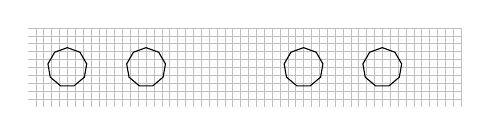
\begin{tikzpicture}[node distance=0pt, every node/.style={outer sep=0pt}]
        \draw [help lines,gray!50,step =0.1] (-0.5,-0.5) grid (5,0.5);
      %\node (1-C1) [my poly=10] {C1};
        \node (poly) [regular polygon, regular polygon sides=9, draw, minimum size = 0.5cm] at (0,0) {};
        \node (poly) [regular polygon, regular polygon sides=9, draw, minimum size = 0.5cm] at (1,0) {};
        \node (poly) [regular polygon, regular polygon sides=9, draw, minimum size = 0.5cm] at (3,0) {};
        \node (poly) [regular polygon, regular polygon sides=9, draw, minimum size = 0.5cm] at (4,0) {};
        %\fill[red] at (0.7, 0.2) circle (1pt);
        %\node[fill=red, minimum size = 0.01cm] at (0.7, -0.2) {};
      %\foreach \i/\j/\k/\m in {4/2/2/30,3/1/3/10,2/6/4/10,1/5/5/10,6/4/6/10,5/3/7/10}
      %\node (1-C\k) [my poly=\m, anchor=corner \i] at (1-C1.corner \j) {C\k};
    \end{tikzpicture}}
\end{figure}

We are done when either each line crosses with another line (point to point) or when we ran out of vertices on a chain, being the closest point the intersection of the perpenciular through the other vertex.

Below, we include a pseudocode snippet for the resolution of this problem. Note that we use an \texttt{external\_tangents} method that we assume implemented (P3).%, and that $P_A$ or $P_B$ can be void at some iteration.
\begin{algorithm}
    \caption{Given two polygons $\mathcal{P}$ and $\mathcal{Q}$, find the closest pair of points, one in $\mathcal{P}$ and the other in $\mathcal{Q}$. \label{alg:closest-poly}}
  \begin{multicols}{2}
  \begin{algorithmic}[1]
    %\Procedure{T-DAG Generation}{$s$}
        \State $s_p, e_p, s_q, e_q \gets \text{external\_tangents}(P, Q)$
        \State $bin_p \gets s_p + \frac{e_p - s_p}{2}$
        \State $bin_q \gets s_q + \frac{e_q - s_q}{2}$
        \While{$s_p \leq bin_p \leq e_p \wedge s_q \leq bin_q \leq e_q $}
            \State $bin_p \gets s_p + \frac{e_p - s_p}{2}$
            \State $bin_q \gets s_q + \frac{e_q - s_q}{2}$
            \State $l_{pA} \gets \text{line}(\perp bin_pbin_{p+1}, bin_p)$
            \State $l_{qA} \gets \text{line}(\perp bin_qbin_{q+1}, bin_q)$
            \State $l_{pB} \gets \text{line}(\perp bin_pbin_{p-1}, bin_p)$ 
            \State $l_{qB} = \text{line}(\perp bin_qbin_{q-1}, bin_q)$
            \Switch{}
                \Case{$l_{pA} \cap l_{qA} \neq \emptyset \& l_{pB} \cap l_{qA} \neq \emptyset$}
                    \State $e_p \gets bin_p$
                \EndCase
                \Case{$l_{pA} \cap l_{qB} \neq \emptyset \& l_{pB} \cap l_{qB} \neq \emptyset$}
                    \State $s_p \gets bin_p$
                \EndCase
                \Case{$l_{pA} \cap l_{qA} \neq \emptyset \& l_{pA} \cap l_{qB} \neq \emptyset$}
                    \State $s_q \gets bin_q$
                \EndCase
                \Case{$l_{pB} \cap l_{qA} \neq \emptyset \& l_{pB} \cap l_{qB} \neq \emptyset$}
                    \State $e_q \gets bin_q$
                \EndCase
                \Case{$l_{pA} \cap l_{qA} \neq \emptyset \& l_{pB} \cap l_{qB} \neq \emptyset$}
                    \State \Return $bin_p, bin_q$
                \EndCase
            \EndSwitch
        \EndWhile
        \If{$!(s_p \leq bin_p \leq e_p)$}
            \State \Return $bin_q, \text{line}(\perp s_pe_p, bin_q) \cap s_pe_p$
        \Else
            \State \Return $bin_p, \text{line}(\perp s_qe_q, bin_p) \cap s_qe_q$
        \EndIf
    %\EndProcedure
  \end{algorithmic}
  \end{multicols}
\end{algorithm}

\textbf{Running Time} Both the tangents and this second algorithm run at most $\log(m) + \log(n)$ iterations hence the complexity of the tangent calculation dominates the running time, being the algorithm in $\mathcal{O}(\log(m) + \log(n))$.

\vfill

\textbf{Note from author} Resolution to problems 4 and 5 was done in this order. However, knowing the answer to 5, one could solve 4 similarly, leaving $p$ fixed and taking the two tangents from $p$ to $\mathcal{P}$ as the reference/perpendicular lines.
\end{document}
